%% ------------------------------------------------------------------------- %%
\chapter{Conceitos}
\label{cap:conceitos}

Texto texto texto texto texto texto texto texto texto texto texto texto texto
texto texto texto texto texto texto texto texto texto texto texto texto texto
texto texto texto texto texto texto texto texto texto texto texto texto texto
texto texto texto texto texto texto texto texto texto texto texto texto texto
texto texto texto texto texto texto.

%% ------------------------------------------------------------------------- %%
\section{Fundamentos}\index{área do trabalho!fundamentos}
\label{sec:fundamentos}

Texto texto texto texto texto texto texto texto texto texto texto texto texto
texto texto texto texto texto texto texto texto texto texto texto texto texto
texto texto texto texto texto texto texto texto texto texto texto texto texto
texto texto texto texto texto texto texto texto texto texto texto texto texto
texto texto texto.

%% ------------------------------------------------------------------------- %%
\subsection{Ácidos Nucléicos}\index{ácido!nucléico}\index{nucleotídeos}
\label{sec:acidos_nucleicos}

Na Figura~\ref{fig:humanbeta} texto texto texto texto texto texto texto texto
texto texto texto texto texto texto texto texto texto texto texto texto texto
texto texto texto texto texto texto texto texto texto texto texto texto texto
texto texto texto texto texto texto texto texto texto texto texto texto texto
texto texto texto.

\begin{figure}[!h]
  \centering
  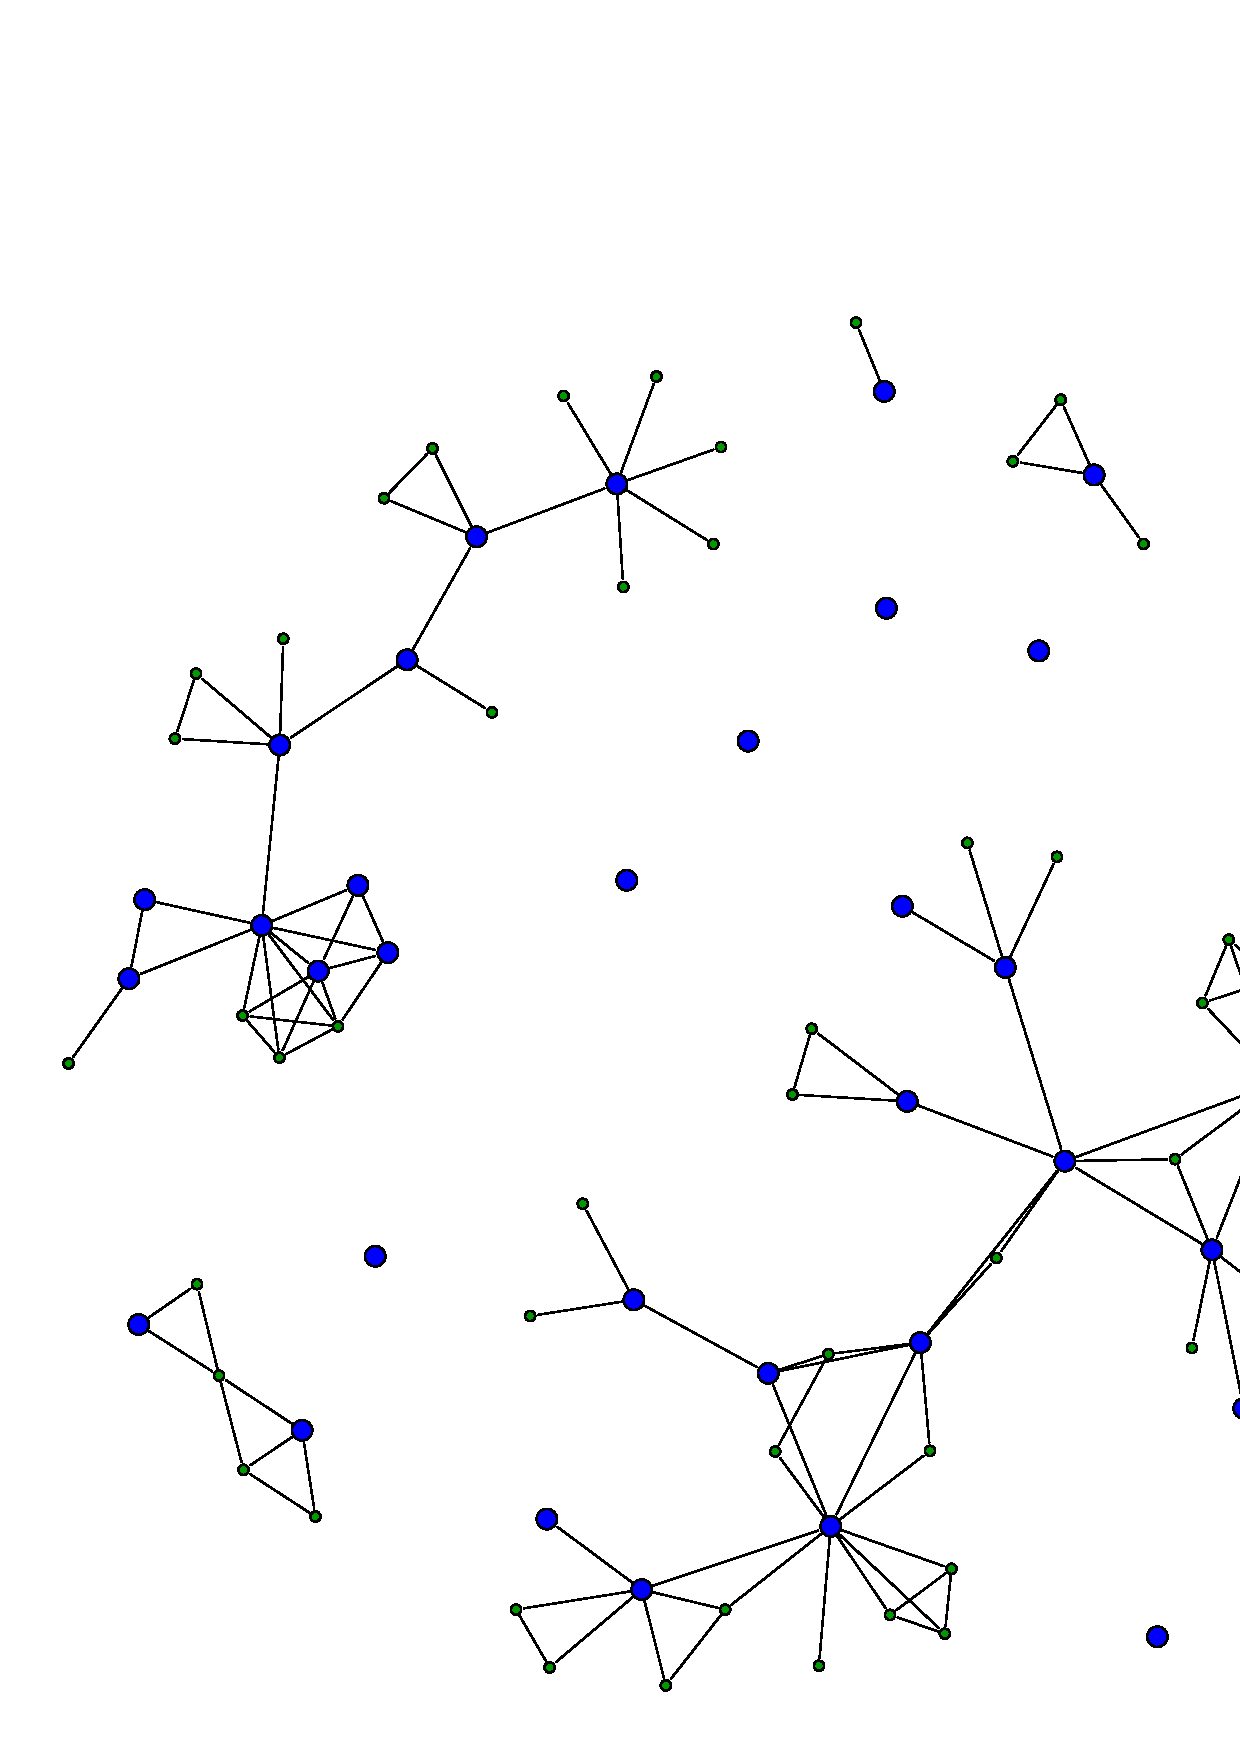
\includegraphics[width=.40\textwidth]{graph} 
  \caption{Descrição da figura mostrada.}
  \label{fig:humanbeta} 
\end{figure}

%% ------------------------------------------------------------------------- %%
\subsection{Aminoácidos}\index{ácido!amino|(}
\label{sec:amino_acidos}

Veja na Tabela \ref{tab:amino_acidos}...  texto texto texto texto texto texto
texto texto texto texto texto texto texto texto texto texto texto texto texto
texto texto texto texto texto texto texto texto texto texto texto texto texto
texto texto texto texto texto texto texto texto texto texto texto texto texto
texto texto texto texto texto texto texto texto texto texto texto.

\begin{table}[!t]
\begin{center}
    \begin{tabular}{c|c|l}
	 \hline
	 Código & Abreviatura & Nome completo \\ \hline
     \texttt{A} & Ala & Alanina \\
     \texttt{C} & Cys & Cisteína \\
     ...        & ... & ... \\
     \texttt{W} & Trp & Tiptofano \\
     \texttt{Y} & Tyr & Tirosina \\ \hline
    \end{tabular}
  \caption{Códigos, abreviaturas e nomes dos aminoácidos.}
  \label{tab:amino_acidos}
\end{center}
\end{table}
\index{ácido!amino|)}

Texto texto texto texto texto texto texto texto texto texto texto texto texto
texto texto texto texto texto texto texto texto texto texto texto texto texto
texto texto texto texto texto texto texto texto texto texto texto texto texto
texto texto texto texto texto texto texto texto texto texto texto texto texto
texto texto texto texto texto texto texto.


%% ------------------------------------------------------------------------- %%
\section{Exemplo de Código-Fonte em Python}
\label{sec:exemplo_codigo_fonte}
Texto texto texto texto texto texto texto texto texto texto texto texto texto
texto texto texto texto texto texto texto texto texto texto texto texto texto
texto texto texto texto texto texto texto texto texto texto texto texto texto
texto texto texto texto texto texto texto.

% Foi utilizado o pacote listing para formatar código fonte
% http://ctan.org/tex-archive/macros/latex/contrib/listings/listings.pdf
% Veja no preambulo do arquivo tese-exemplo.tex os parâmetros de configuração.

\begin{lstlisting}[frame=trbl]
   def puralize(words):
   result = []
   for word in words:
       word = words[i]
       if word.endswith('s') or word.endswith('x'):
           plural = word + 'es')
       if word.endswith('y'):
           plural = word[:-1] + 'ies'
       else:
           plural = +  's'
       result.append(plural)
    return result
\end{lstlisting}


%% ------------------------------------------------------------------------- %%
\section{Algumas Referências}
\label{sec:algumas_referencias}

É muito recomendável a utilização de arquivos \emph{bibtex} para o gerenciamento
de referências a trabalhos. Nesse sentido existem três plataformas gratuitas
que permitem a busca de referências acadêmicas em formato bib: 
\begin{itemize}
	\item \emph{CiteULike} (patrocinados por Springer): \url{www.citeulike.org}
	\item Coleção de bibliografia em Ciência da Computação: \url{liinwww.ira.uka.de/bibliography}
	\item Google acadêmico (habilitar bibtex nas preferências): \url{scholar.google.com.br}
\end{itemize}
Lamentavelmente, ainda não existe um mecanismo de verificação ou validação das
informações nessas plataformas. Portanto, é fortemente sugerido validar todas
as informações de tal forma que as entradas bib estejam corretas.  Também, tome
muito cuidado na padronização das referências bibliográficas: ou considere TODOS
os nomes dos autores por extenso, ou TODOS os nomes dos autores abreviados.
Evite misturas inapropriadas.

Exemplos de referências com a tag:
\begin{itemize}
\item @Book: \cite{JW82}.
{\scriptsize\begin{verbatim}
@Book{JW82,
 author   = {Richard A. Johnson and Dean W. Wichern},
 title    = {Applied Multivariate Statistical Analysis},
 publisher= {Prentice-Hall},
 year     = {1983}
}
\end{verbatim}}

\item @Article: \cite{MenaChalco08}.
{\scriptsize\begin{verbatim}
@Article{MenaChalco08,
 author   = {Jesús P. Mena-Chalco and Helaine Carrer and Yossi Zana and 
            Roberto M. Cesar-Jr.},
 title    = {Identification of protein coding regions using the modified 
            {G}abor-wavelet transform},
 journal  = {IEEE/ACM Transactions on Computational Biology and Bioinformatics},
 volume   = {5},
 pages    = {198-207},
 year     = {2008},
}
\end{verbatim}}

\item @InProceedings: \cite{alves03:simi}.
{\scriptsize\begin{verbatim}
@InProceedings{alves03:simi,
 author   = {Carlos E. R. Alves and Edson N. Cáceres and Frank Dehne and 
            Siang W. Song},
 title    = {A Parallel Wavefront Algorithm for Efficient Biological 
            Sequence Comparison},
 booktitle= {ICCSA '03: The 2003 International Conference on Computational Science
            and its Applications},
 year     = {2003},
 pages    = {249-258},
 month    = May,
 publisher= {Springer-Verlag}
}
\end{verbatim}}

\item @InCollection: \cite{bobaoglu93:concepts}.
{\scriptsize\begin{verbatim}
@InCollection{bobaoglu93:concepts,
 author   = {Ozalp Babaoglu and Keith Marzullo},
 title    = {Consistent Global States of Distributed Systems: Fundamental Concepts
            and Mechanisms},
 editor   = {Sape Mullender},
 booktitle= {Distributed Systems},
 edition  = {segunda},
 year     = {1993},
 pages    = {55-96}
}
\end{verbatim}}

\item @Conference: \cite{bronevetsky02}.
{\scriptsize\begin{verbatim}
@Conference{bronevetsky02,
 author   = {Greg Bronevetsky and Daniel Marques and Keshav Pingali and 
            Paul Stodghill},
 title    = {Automated application-level checkpointing of {MPI} programs},
 booktitle= {PPoPP '03: Proceedings of the 9th ACM SIGPLAN Symposium on Principles
            and Practice of Parallel Programming},
 year     = {2003},
 pages    = {84-89}
}
\end{verbatim}}

\item @PhdThesis: \cite{garcia01:PhD}.
{\scriptsize\begin{verbatim}
@PhdThesis{garcia01:PhD,
 author   = {Islene C. Garcia},
 title    = {Visões Progressivas de Computações Distribuídas},
 school   = {Instituto de Computação, Universidade de Campinas, Brasil},
 year     = {2001},
 month    = {Dezembro}
}
\end{verbatim}}

\item @MastersThesis: \cite{schmidt03:MSc}.
{\scriptsize\begin{verbatim}
@MastersThesis{schmidt03:MSc,
 author   = {Rodrigo M. Schmidt},
 title    = {Coleta de Lixo para Protocolos de \emph{Checkpointing}},
 school   = {Instituto de Computação, Universidade de Campinas, Brasil},
 year     = {2003},
 month    = Oct
}
\end{verbatim}}

\item @Techreport: \cite{alvisi99:analysisCIC}.
{\scriptsize\begin{verbatim}
@Techreport{alvisi99:analysisCIC,
 author   = {Lorenzo Alvisi and Elmootazbellah Elnozahy and Sriram S. Rao and
            Syed A. Husain and Asanka Del Mel},
 title    = {An Analysis of Comunication-Induced Checkpointing},
 institution= {Department of Computer Science, University of Texas at Austin},
 year     = {1999},
 number   = {TR-99-01},
 address  = {Austin, {USA}}
}
\end{verbatim}}

\item @Manual: \cite{CORBA:spec}.
{\scriptsize\begin{verbatim}
@Manual{CORBA:spec,
 title    = {{CORBA v3.0 Specification}},
 author   = {{Object Management Group}},
 month    = Jul,
 year     = {2002},
 note     = {{OMG Document 02-06-33}}
}
\end{verbatim}}

\item @Misc: \cite{gridftp}.
{\scriptsize\begin{verbatim}
@Misc{gridftp,
 author   = {William Allcock},
 title    = {{GridFTP} protocol specification. {Global Grid Forum}
            Recommendation ({GFD}.20)},
 year     = {2003}
}
\end{verbatim}}

\item @Misc: para referência a artigo online \cite{fowler04:designDead}.
{\scriptsize\begin{verbatim}
@Misc{fowler04:designDead,
 author   = {Martin Fowler},
 title    = {Is Design Dead?},
 year     = {2004},
 month    = May,
 note     = {Último acesso em 30/1/2010},
 howpublished= {\url{http://martinfowler.com/articles/designDead.html}},
}
\end{verbatim}}

\item @Misc: para referência a página web \cite{FSF:GNU-GPL}.
{\scriptsize\begin{verbatim}
@Misc{FSF:GNU-GPL,
 author   = {Free Software Foundation},
 title    = {GNU general public license},
 note     = {Último acesso em 30/1/2010},
 howpublished= {\url{http://www.gnu.org/copyleft/gpl.html}},
}
\end{verbatim}}

\end{itemize}

